
\subsection{Worst-case bit patterns}

The worst-case bit pattern for the channel running at 10Gb/s was generated by rendering the pulse response of the channel using the convolution of a 100ps pulse and the impulse response of the channel. A truncated plot of the resulting output is depicted in figure \ref{fig:worst}.


\begin{figure}[ht!]
\begin{center}
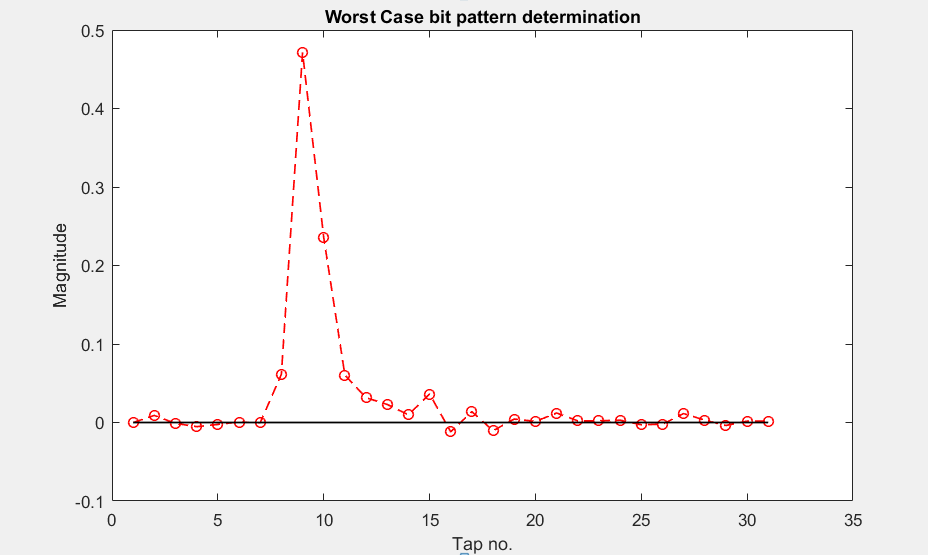
\includegraphics[scale=0.8]{img/graph}
\caption{Truncated pulse reponse of the channel, with the cursors marked as 'o's.}
\label{fig:worst}
\end{center}
\end{figure}

From the pulse response the worst-case bit pattern for transmitting a 
'1' was determined using the method learned in class, which is to flip the pulse response vertically and then using the highest peak as the cursor and each point an UI away as post/pre-cursors. If a post/pre-cursor has a positive value the corresponding bit in the pattern should be a '0', and a negative value yields a '1'.

The resulting worst-case bit pattern for a '1' around the cursor is shown in figure \ref{eq:wc}, where the cursor is the underlined '1'. The worst-case bit pattern for a '0' can be obtained by negating the bit-sequence for the worst-case '1'.


\begin{figure}

$$\left[0,1,1,0,0,0,0,0,0,1,0,1,0,0,0,0,0,0,1,0,\underline{1},0,1,1,1,0,1,1,1,1,1,1,1,1,1,1,1,1,1,1,1,1\right]$$
\caption{Worst-case bit pattern for transmitting a '1' on the transmission line, the cursor is the underlined '1' in the pattern.}
\label{eq:wc}

\end{figure}



The used method yields the worst-case bit pattern with regard to eye-height, a worst-case bit pattern can also be determined to test the eye-width, this is described in ~\cite{designcon2011a}.

If worst-case bit-patterns for the other speeds of the transmission line are wanted, rendering it is a matter of using a different length pulse and use the UI for that pulse to determine the taps.